\section{Computational methods}
\label{sec:methods}

\subsection{Interface cell}
\label{sec:cell}

All calculations were performed with LAMMPS (22~Jul~2025 release, KOKKOS/CUDA
build for graphics processors) \cite{Thompson2022LAMMPS}. Interatomic forces
are given by the 2NN-MEAM potential (second-nearest-neighbour modified
embedded-atom method) of Jelinek \emph{et al.} for the Al--Si--Mg--Cu--Fe
system \cite{Jelinek2012}, a single potential that describes every atom in
the cell, including the atoms on either side of the interface, by one set of
interaction rules.

The matrix is face-centred cubic (fcc) aluminium ($a=4.05$~\AA{}). Its
orientation, $x\parallel[1\bar{1}0]$, $y\parallel[11\bar{2}]$,
$z\parallel[111]$, is dictated by the slip system of fcc Al: dislocations in
aluminium move on $\{111\}$ planes along $\langle110\rangle$ directions, and
with this choice the (111) glide plane is parallel to the interface and the
$[1\bar{1}0]$ glide direction lies along $x$. An edge dislocation (the edge
of an extra half-plane of atoms inserted into the crystal) with Burgers
vector $\tfrac{1}{2}[1\bar{1}0]$---the lattice translation that measures the
displacement it carries, $|\mathbf{b}|=2.86$~\AA{}---and line along $y$ then spans the whole width of the cell, so that it
represents an infinitely long straight dislocation, and glides in $x$
parallel to the interface,
which is the motion the mechanism under test would have to produce.

The inclusion is the monoclinic intermetallic Al$_{13}$Fe$_4$ in the
structure of Ref.~\cite{Liu2024CIF}. It is built as a flat layer 20~\AA{}
thick that carries on its upper surface a half-elliptical bulge (referred to
below as the ridge) with semi-axes 35~\AA{} along $x$ and 20~\AA{} along $z$,
running the full length of the cell along $y$. The ridge is essential: a
flat strained layer that spans the entire cell can relieve its normal stress
simply by expanding upward, and it is the curved edges of the ridge that
produce a non-uniform stress field in the matrix, as the curvature of the
surface of a real particle would. The flat layer is left unstrained and the ridge alone carries the strain
(Section~\ref{sec:eigenstrain}).

In $x$ and $y$ the cell is periodic: an atom leaving through one face
re-enters through the opposite face, so the cell represents an interface
unbounded in its plane. The in-plane dimensions ($L_x=154.64$~\AA{}, $L_y=64.48$~\AA{}: 54 and 13
periods of the aluminium lattice, ten and eight cells of Al$_{13}$Fe$_4$) are
chosen so that both lattices are periodic in the plane. The small residual
mismatch ($-0.22\%$ along $x$, $-0.26\%$ along $y$) is taken up by the
inclusion and is the same in the strained and in the control cell, so that it
cancels to first order when the two are compared. Aluminium atoms lying within
2.2~\AA{} of an inclusion atom (periodic images included) are removed; the
smallest interatomic distance in the resulting structure is 2.22~\AA{}. The
aluminium layer above the interface plane is 129~\AA{} thick (56 atomic (111)
planes), the whole cell contains 91\,428 atoms (72\,532 in the matrix and
18\,896 in the inclusion), and in $z$ it is bounded by a free surface with
17~\AA{} of vacuum above it and by a layer 6~\AA{} thick at the bottom whose
atoms are held fixed (Fig.~\ref{fig:cell}).

The inclusion is bonded to the matrix. Atoms on both sides of the interface
interact through the same potential, no constraint or artificial coupling is
imposed at the interface, and the interface neither slips nor opens except
through the atomic displacements the potential itself allows. The control structure is relaxed in three stages: energy minimisation by
conjugate gradients (the atoms are moved to positions of minimum energy
without thermal motion), 6~ps of molecular dynamics at 300~K followed by
12~ps of cooling to 0.5~K, which relax the long-wavelength modes of the slab
that minimisation alone does not reach, and a final minimisation to a force
of 0.05~eV/\AA{} (two-norm over all atoms). The strained cell is built from
this relaxed state (Section~\ref{sec:eigenstrain}) and minimised to
0.02~eV/\AA{}.

\begin{figure}
\centering
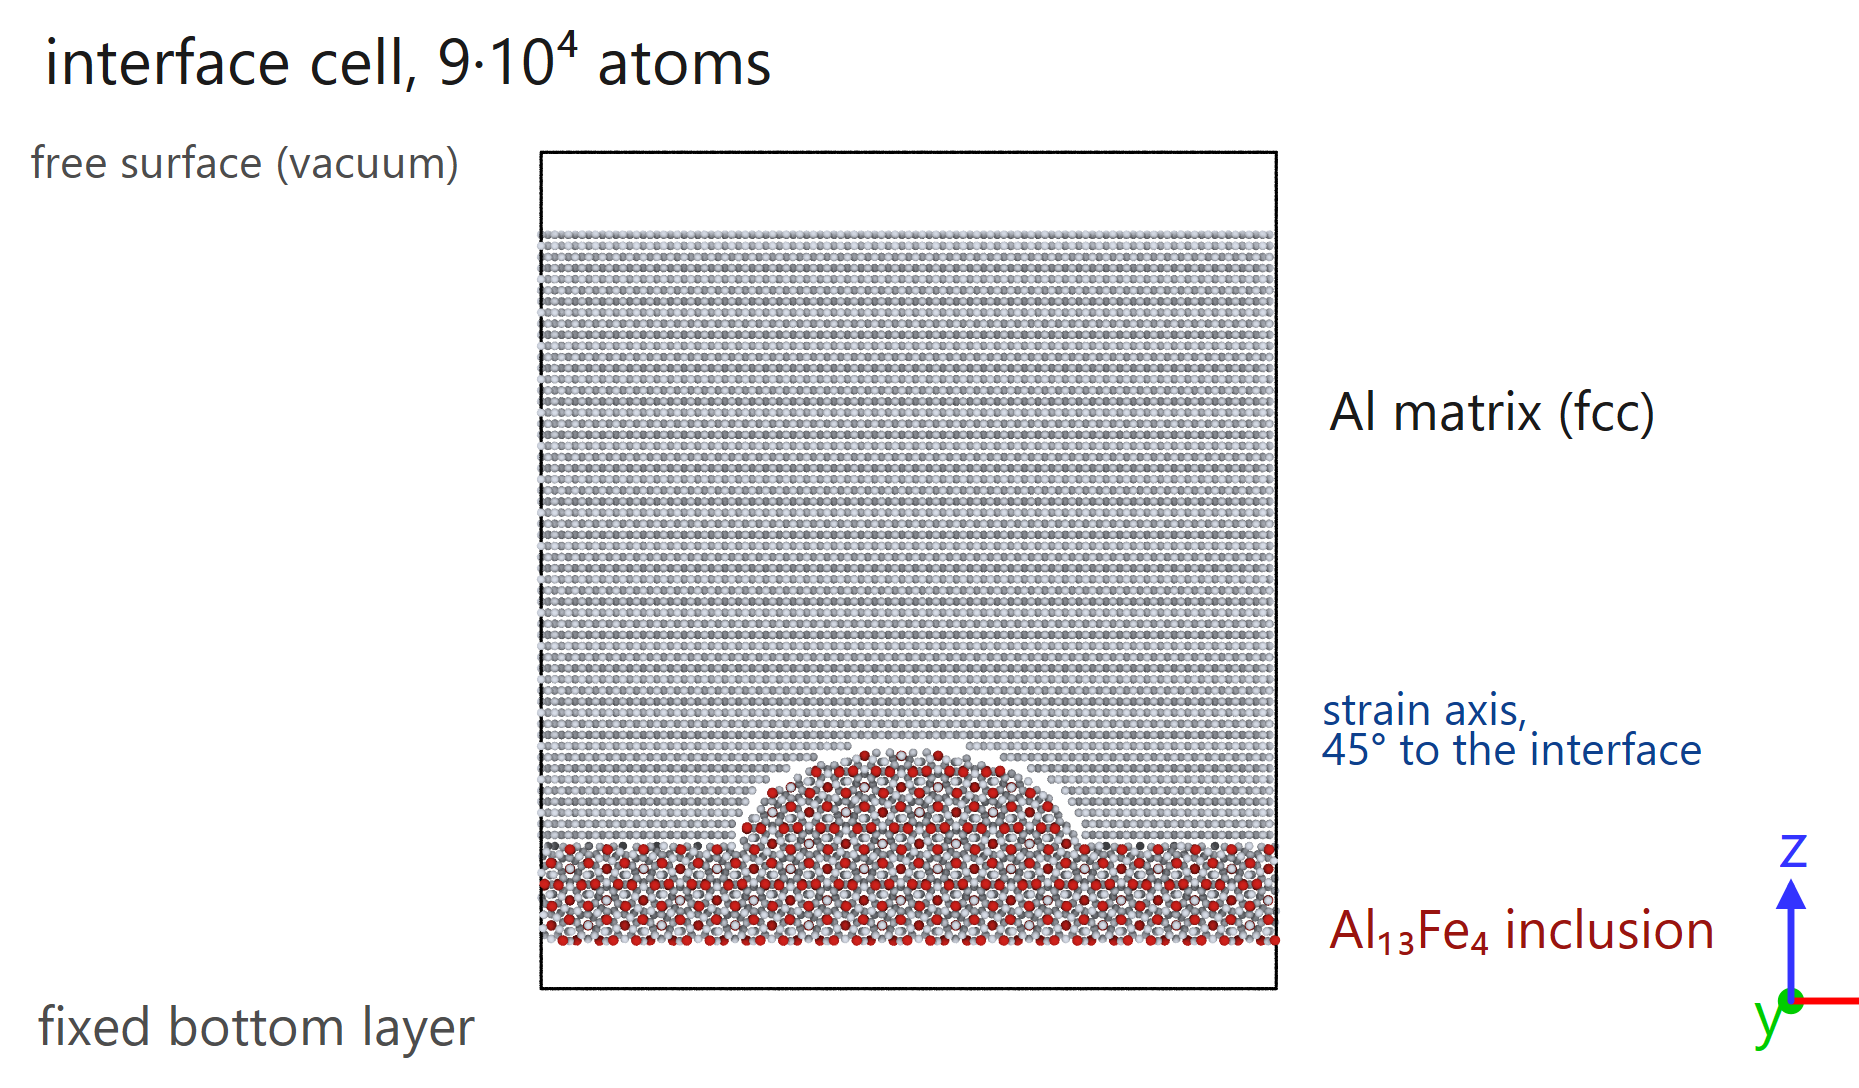
\includegraphics[width=0.92\linewidth]{fig_cell_interface_en}
\caption{The interface cell, viewed along $y$ (the $x$--$z$ plane). Grey:
the aluminium matrix, 129~\AA{} of fcc aluminium with $x=[1\bar{1}0]$,
$y=[11\bar{2}]$ and $z=[111]$, so that the interface is parallel to a (111)
glide plane and $x$ is a glide direction. Red: the Al$_{13}$Fe$_4$ inclusion,
a flat layer with a half-elliptical ridge 70~\AA{} wide and 20~\AA{} high.
The lowest 6~\AA{} of the inclusion are held fixed; above the aluminium is
vacuum. The cell is periodic along $x$ and $y$. The imposed elongation of the
inclusion is directed at $45^{\circ}$ to the interface in the $x$--$z$
plane.}
\label{fig:cell}
\end{figure}

\subsection{Representation of the field}
\label{sec:eigenstrain}

Molecular dynamics is classical mechanics, and the magnetic field itself is
not present in the calculation. Its action is represented mechanically, by
the strain it is assumed to produce in the inclusion. Following the earlier
experimental studies
\cite{Skvortsov2019JAP,Skvortsov2019PSS,Friha2024JMMM,Nikolaev2025SciRep},
in which the field acts through magnetostriction, i.e. the elongation of the
inclusion along the direction of the field, the inclusion is taken to
elongate along the field direction $\mathbf{u}$ by
$\varepsilon=1.94\times10^{-3}$ (0.194\%), the elastic strain
$\sigma_m/E_{\mathrm{Al}}$ (with $E_{\mathrm{Al}}=75.7$~GPa) corresponding to
the interface stress $\sigma_m=147$~MPa estimated in those works
\cite{Friha2024JMMM}, at constant volume: elongation $\varepsilon$ along $\mathbf{u}$ and contraction
$\varepsilon/2$ along the two perpendicular directions. Written as a tensor,
\begin{equation}
\varepsilon^{*}_{ij}
  =\tfrac{3}{2}\,\varepsilon\!\left(u_i u_j-\tfrac{1}{3}\delta_{ij}\right),
\qquad \operatorname{tr}\varepsilon^{*}=0,
\label{eq:eigenstrain}
\end{equation}
where $\delta_{ij}$ equals 1 for $i=j$ and 0 otherwise and the zero trace
expresses the constancy of volume. In the elasticity of inclusions a strain
of this kind, the one the inclusion would adopt if it were free of the
matrix, is called an eigenstrain \cite{Eshelby1957}; the term is used below
in that sense. The value adopted is well above the magnetostriction measured
in Fe--Al alloys \cite{Hall1959,BormioNunes2012}; it is used because it is
the amplitude the proposed mechanism itself presupposes, and the mechanism
is tested at that amplitude.

The direction $\mathbf{u}$ is inclined at $45^{\circ}$ to the interface
normal, in the $x$--$z$ plane. The reason is geometric. For $\mathbf{u}$
along the normal $z$ the imposed strain produces no shear stress at all on
the $(111)[1\bar{1}0]$ glide system: the Schmid factor (the geometric factor
that converts a stress into the shear stress acting on a given slip system)
is exactly zero, and no force whatever would act on a dislocation gliding
parallel to the interface. At $45^{\circ}$ the shear component of the
imposed strain on the glide plane is at its maximum,
$\varepsilon^{*}_{xz}=\tfrac{3}{4}\varepsilon=1.46\times10^{-3}$. In a
polycrystal the grains that respond to the field are those whose slip planes
are favourably inclined to it, and the tilted cell represents that
population. The tilt is the same in every cell.

The strain is applied by displacing every atom of the ridge relative to the
centre of the ridge in proportion to its position,
$\mathbf{r}\rightarrow\mathbf{r}+\varepsilon^{*}\!\cdot\!\mathbf{r}$, which
stretches the ridge uniformly along $\mathbf{u}$ and compresses it across
$\mathbf{u}$. The flat layer beneath the ridge is left unstrained. It spans
the periodic cell, and a layer that is periodic in its plane cannot be
sheared coherently: held at the shear of Eq.~(\ref{eq:eigenstrain}) its
surface would be a sawtooth with a step of $\varepsilon^{*}_{xz}L_x=0.22$~\AA{}
at the cell boundary, and the whole aluminium slab above it would be
stretched along $z$ by about $\varepsilon^{*}_{xz}$---a stress of order
150~MPa across the cell, which is what was observed when this was tried. The
ridge is the particle whose field is measured; the layer only closes the
cell. The interatomic potential is not modified. The stress field
produced by the strained inclusion is obtained as the difference between a
cell with the strained inclusion and a control cell without strain, both
minimised from identical starting structures under identical conditions. Two
variants are computed, differing in whether the inclusion is allowed to
relax.

In the \emph{maintained} case every inclusion atom---the ridge at its
displaced position, the flat layer at its original one---is held by a stiff
spring (stiffness 20~eV/\AA$^{2}$, which keeps the atom within about
0.01~\AA{} of that position) while the matrix relaxes around it, so that the
ridge holds the strain of Eq.~(\ref{eq:eigenstrain}) throughout. The springs
are attached in the same way in the corresponding control cell, so they
cancel in the difference between the two. This cell gives the stress field
of a particle that maintains its eigenstrain.
Under the forces that arise at the interface the inclusion atoms depart from
their strained positions by about 0.01~\AA{}, and the ridge retains
$0.97\pm0.004$ of the imposed strain (measured as described for the free case
below).

In the \emph{free} case no springs are attached and the inclusion is free to
relax the imposed strain back out. It does so to a large extent: after
minimisation the ridge, which produces the field measured in the matrix,
retains 0.2--0.4 of the imposed strain ($0.20\pm0.11$ and $0.44\pm0.10$ in
two minimisations, both stopped before full convergence). The fraction is measured as the
projection of the residual distortion of the Fe sublattice of the inclusion
onto $\varepsilon^{*}$, obtained by a least-squares fit of the displacements
between the strained and the control cell; the uncertainty is the standard
error of that fit. The free cell shows what an inclusion does when nothing
holds its strain; its stress field is the relaxed response, not the field of
an inclusion that maintains the strain, and it is the maintained case that is
compared with the dislocation thresholds below.

The \emph{control} cell has no strain. It is the relaxed structure of
Section~\ref{sec:cell} itself; the strained cell is built from it, minimised
with the same tolerance and compared with it atom by atom, so that the
residual lattice mismatch of Section~\ref{sec:cell}, the arrangement of the
interfacial layer and the long-wavelength strain of the slab are common to
both and cancel in the difference. The interface cells supply the stress profile in the
matrix and its decay length. The stresses at which dislocations begin to move
are obtained separately, in the loaded cells of Section~\ref{sec:loading},
and serve only as the thresholds against which that profile is compared.

\subsection{Loaded cells and loading scheme}
\label{sec:loading}

The stresses at which dislocations move are measured in two cells loaded in
shear under dynamics at 300~K.

The first is the interface cell of Section~\ref{sec:cell} with a
pre-existing pair of edge dislocations placed next to the ridge of the
inclusion, 91\,428 atoms in all (Fig.~\ref{fig:loading}). The pair is
a dislocation dipole: two parallel dislocations of opposite sign whose stress
fields attract, so that in a uniform, stress-free crystal the pair is stable and stays where it is placed until
the applied stress exceeds the level at which the two partners can pass each
other. Both dislocations lie along $y$ and glide on (111) planes parallel to
the interface. The partners are offset by 23.4~\AA{} along $x$ and by ten
(111) interplanar spacings, 23.4~\AA{}, along $z$, so that the line joining
them is inclined at $45^{\circ}$ to the glide planes. Two edge dislocations
of opposite sign on glide planes a distance $h$ apart attract with a shear
stress of up to $\mu b/[8\pi(1-\nu)h]$, which for $h=23.4$~\AA{} is 198~MPa
(with $\mu=26.5$~GPa, $\nu=0.347$ and $b=2.864$~\AA{}); this is the applied
stress at which they would pass each other in an unbounded crystal. The lower
partner is placed 27~\AA{} beyond the foot of the ridge and 29~\AA{} above the
interface plane, the upper one 23~\AA{} higher and 23~\AA{} closer to the
ridge. The cell is loaded by a shear stress raised
linearly from 0 to 400~MPa over 96~ps, after 5~ps at zero stress. The stress
is applied as a uniform force along $x$ on the atoms of the top atomic
layers, with the reaction taken by the fixed bottom layer; the rate of rise
is switched on smoothly over the first 16~ps so that the lowest shear
vibration of the slab is not excited. The loading is far faster than any
laboratory test (an effective strain rate of order $10^{8}$~s$^{-1}$), so the
thresholds obtained are upper estimates relative to slow loading. Three ramps were run: the unstrained cell with the inclusion free to relax,
to 400~MPa over 96~ps; and the unstrained and the strained cell with the
inclusion held by the springs of Section~\ref{sec:eigenstrain}, at the same
rate of rise, to 145~MPa over 40~ps---the pair that compares strained with
unstrained.

The second cell has no inclusion. It is a slab of the alloy matrix with the
same orientation, 92\,800 atoms (91\,315~Al, 928~Mg, 557~Si; $114.6\times49.6\times291$~\AA{}), in which
1.0~at.\%~Mg and 0.6~at.\%~Si are placed at random on lattice sites, and
which contains one edge dipole whose partners lie 206~\AA{} apart on parallel
glide planes; their mutual attraction corresponds to a shear stress
$\mu b/[8\pi(1-\nu)h]\approx22$~MPa, small compared with the stresses
applied. Before loading, the structure is energy-minimised and brought to
300~K. This cell is loaded in steps: constant shear stresses of 45, 55, 65
and 75~MPa, each held for 30~ps and each switched on smoothly over 4~ps,
after 10~ps at zero stress. Steps are used rather than a ramp because a
dislocation held by solute atoms moves by breaking away from them, a
thermally activated event whose waiting time depends on the stress; holding
the stress constant for a fixed time tests whether the dislocation breaks
away at that level, and the stress is raised in steps to find the level at
which it does. A pure-aluminium cell of the same geometry provides the
solute-free reference.

In both cells the equations of motion are integrated with a time step of
1~fs, about a hundredth of the period of an atomic vibration. The temperature
is held at 300~K by a Nos\'e--Hoover thermostat (damping time 0.1~ps), which
keeps the average kinetic energy of the unconstrained atoms at the set value
by a weak feedback on their velocities. The dislocations are inserted by the
Volterra construction, in which the crystal is cut along a half-plane, the
two faces are displaced relative to each other by one Burgers vector and
rejoined, with the displacement field made compatible with the periodic
cell. The dislocation content of every starting structure is verified with
the dislocation extraction algorithm (DXA) \cite{Stukowski2012DXA}, which
locates dislocation lines in an atomic configuration and determines their
Burgers vectors, as implemented in OVITO \cite{Stukowski2010OVITO}.

\begin{figure}
\centering
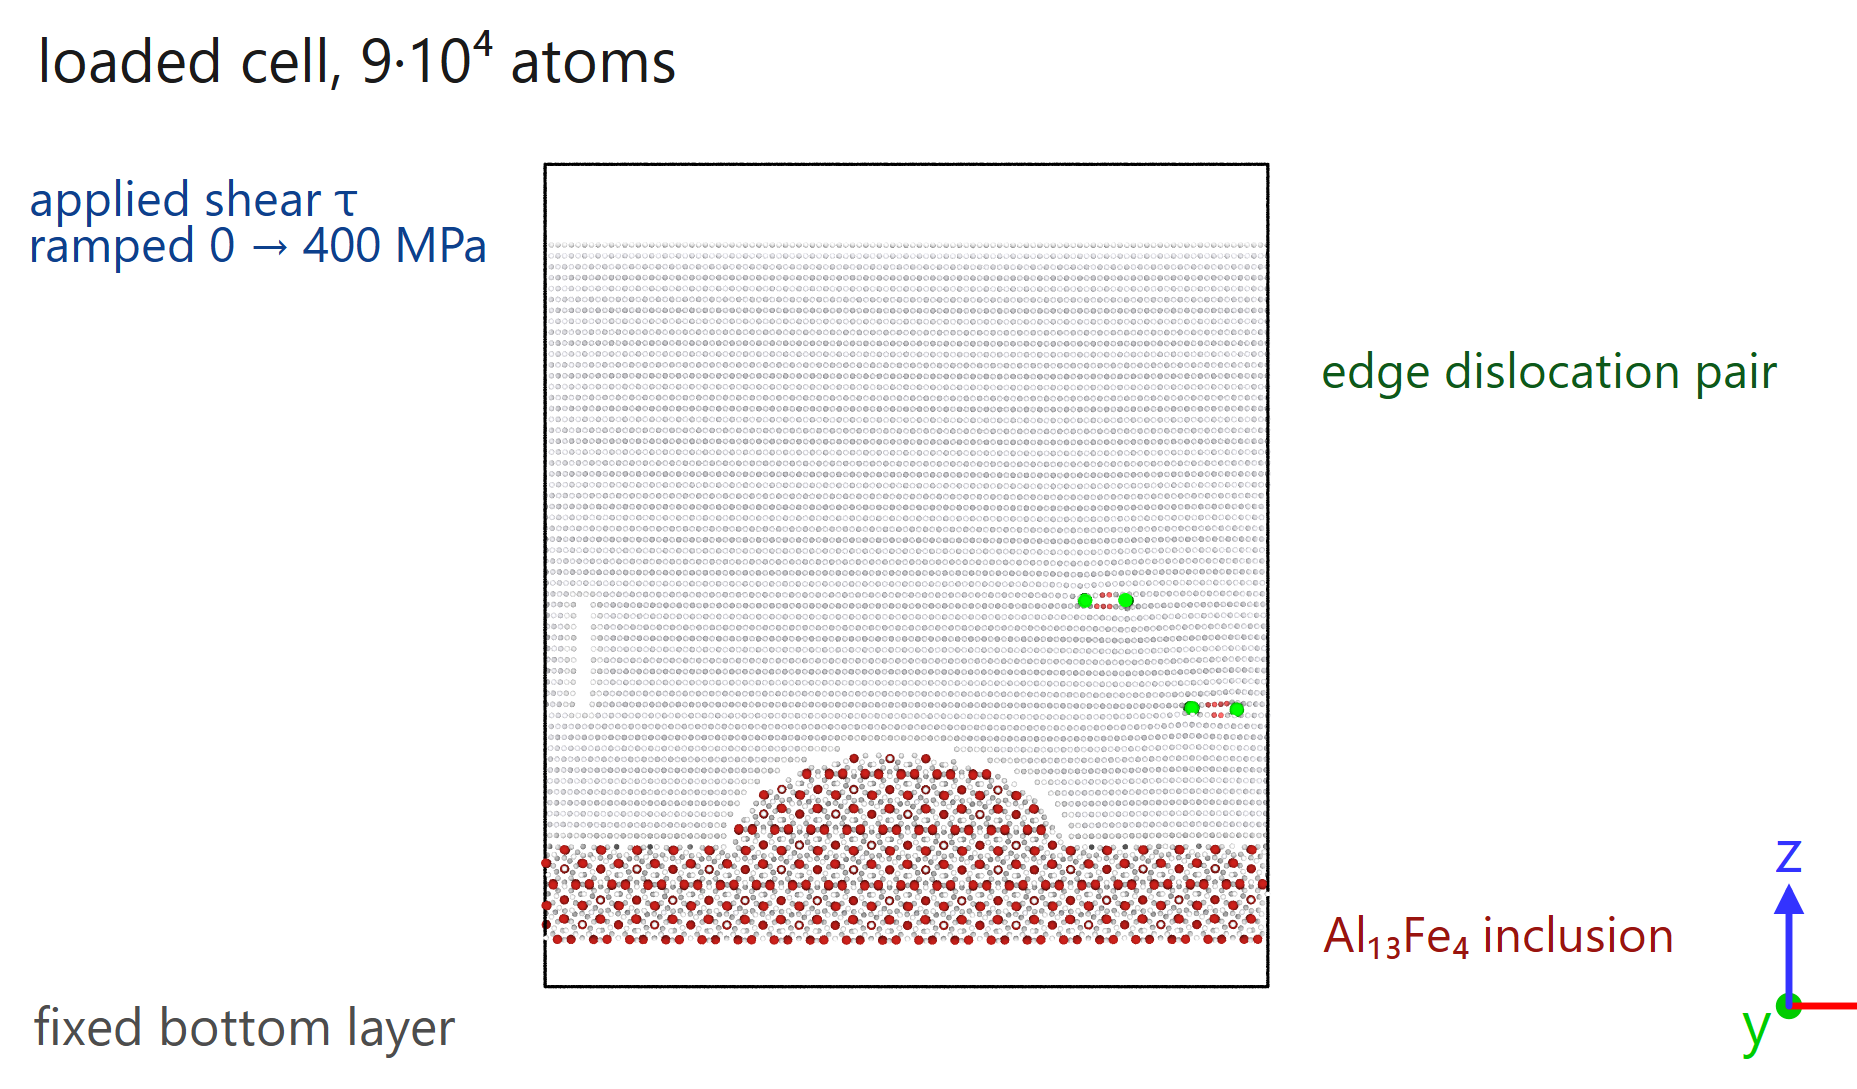
\includegraphics[width=0.92\linewidth]{fig_cell_loading_en}\\[2mm]
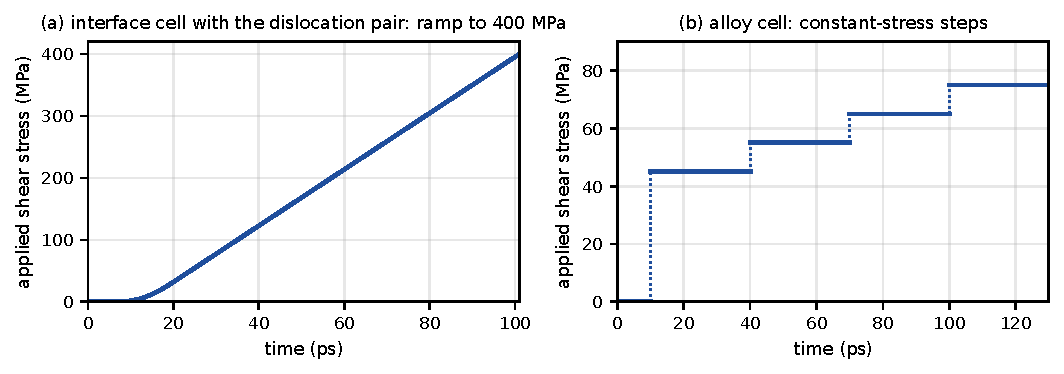
\includegraphics[width=0.92\linewidth]{fig_loading_programme_en}
\caption{The loaded interface cell (top) and the two loading programmes
(bottom). Top: the cell of Fig.~\ref{fig:cell} with a pair of edge
dislocations of opposite sign next to the ridge (green: the dislocation lines
found by dislocation analysis; atoms of the perfect lattice are faded), both
on (111) glide planes parallel to the interface. A shear stress $\tau$ along
$x$ is applied through a uniform force on the top atomic layers and is taken
up by the fixed bottom layer. Bottom: the stress programmes---for this cell a
linear rise from 0 to 400~MPa over 96~ps after 5~ps at zero stress (the
held cells were ramped at the same rate to 145~MPa) (a); for
the alloy cell without inclusion (Section~\ref{sec:mobility}) steps of 45,
55, 65 and 75~MPa, 30~ps each, after 10~ps without load (b).}
\label{fig:loading}
\end{figure}

\subsection{Stress evaluation}
\label{sec:stress}

Local stresses are obtained from the per-atom virial stress, the atomic-scale
counterpart of mechanical stress, computed for each atom from the forces
between it and its neighbours and divided by the atomic volume
$\Omega=16.61$~\AA$^{3}$: $\sigma_{ij}=-\langle W_{ij}\rangle/\Omega$. The
stress of a single atom fluctuates thermally by several GPa, so no scalar
measure is ever formed atom by atom. The six components of the tensor are
first averaged over a slice 4~\AA{} thick parallel to the interface (and, in
the dynamic runs, over time frames), and only then are two scalar measures
formed from the averaged tensor: the von Mises stress, a single positive number that measures the shear
content of a stress state and enters the yield criterion of a ductile metal,
and the resolved shear stress,
the shear stress acting on a given slip plane in a given slip direction.
$\mathrm{RSS}_{\max}$ denotes the largest resolved shear stress among the
twelve $\{111\}\langle110\rangle$ slip systems of the matrix, i.e. the shear
stress on the most favourably oriented system.

Stress profiles $\sigma(r)$ are built as functions of the distance $r$ from
the interface plane in slices 4~\AA{} thick, using only matrix atoms that lie
above the crest of the ridge, so that $r$ measures the distance from the
inclusion surface. The field of the strained inclusion is the difference
between the strained and the control cell, slice by slice. On energy-minimised
structures there is no thermal motion, and the noise level of that difference
is set by the residual slice-to-slice scatter far from the interface: over
$r\geq60$~\AA{} the mean of $\Delta\mathrm{RSS}_{\max}$ is $2.5\pm0.5$~MPa
(mean and standard deviation over thirteen slices), the resolution of the
calculation, below which no field is resolved.